\chapter{Literature review}
\label{mathchapter}

\section{Background}
This section of the thesis focuses on the literature review conducted before starting the development process. It includes a short write-up and a critical analysis of the previous works on the objective proposed in the thesis. There is a comparison drawn between different works based on standard benchmarks used in the industry.
\section{Key related research}
Various works were reviewed and analysed related to the objectives stated in the theses. These are listed below:\\
\begin{itemize}
	\item ArcFace: Additive Angular Margin Loss for Deep Face Recognition 
(9 Feb 2019)
	\item Mis-classified Vector Guided Softmax Loss for Face Recognition
(26 Nov 2019)
	\item LinCos-Softmax: Learning Angle-Discriminative Face Representations With Linearity-Enhanced Cosine Logits
 (15 June 2020)
\end{itemize}
\section{Analysis}
The above works were carefully analysed before moving forward.
All the papers to be discussed propose different loss functions for the classification problem of faces into classes. They tend to minimize intra-class variations and maximize inter-class distances. All the loss functions are just small variations of softmax loss. Accordingly, a short analysis for each paper is stated below:
\\
\begin{itemize}
	\item \textbf{ArcFace: Additive Angular Margin Loss for Deep Face Recognition} : The idea is to add an additive angular margin penalty m between X\textsubscript{i} and W\textsubscript{yi} to simultaneously enhance the intra-class compactness and inter-class discrepancy. This additive angular margin penalty is equal to the geodesic distance margin penalty in the normalised hypersphere.
	\begin{figure}[!h]
    		\centering
    		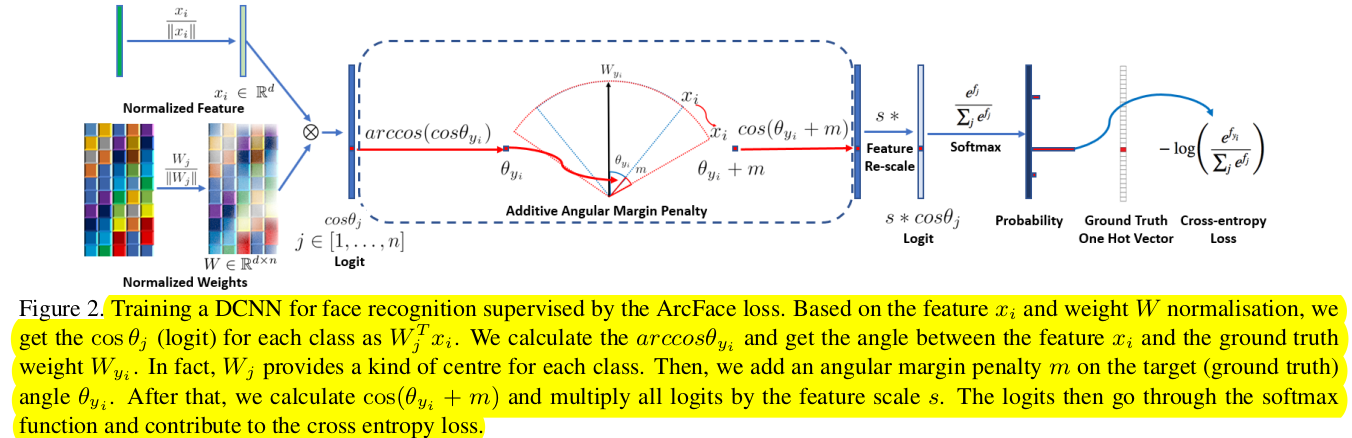
\includegraphics[width=\textwidth]{arcFace}
    		\caption{Source: ArcFace: Additive Angular Margin Loss for Deep Face Recognition}
	\end{figure}
Loss: \begin{equation}
L_{3}=-\frac{1}{N} \sum_{i=1}^{N} \log \frac{e^{s\left(\cos \left(\theta_{y_{i}}+m\right)\right)}}{e^{s\left(\cos \left(\theta_{y_{i}}+m\right)\right)}+\sum_{j=1, j \neq y_{i}}^{n} e^{s \cos \theta_{j}}}
\end{equation}
	\item \textbf{Mis-classified Vector Guided Softmax Loss for Face Recognition} : This paper tries to design a new loss function, which explicitly indicates the hard examples as mis-classified vectors and adaptively emphasizes on them to guide the discriminative feature learning.
As a consequence, our new loss also absorbs the discrimiantibility from other non-ground truth classes as well as is with adaptive margins for different classes.This paper defines a binary indicator I\textsubscript{k} to adaptively indicate whether a sample (feature) is mis-classified by a specific classifier w\textsubscript{k} (where k != y) in the current stage:
\begin{equation}
I_{k}=\left\{\begin{array}{ll}
0, & f\left(m, \theta_{\boldsymbol{w}_{y}, x}\right)-\cos \left(\theta_{\boldsymbol{w}_{k}, x}\right) \geq 0 \\
1, & f\left(m, \theta_{\boldsymbol{w}_{y}, x}\right)-\cos \left(\theta_{\boldsymbol{w}_{k}, x}\right)<0
\end{array}\right.
\end{equation}
Loss:
\begin{equation}
\mathcal{L}_{5}=-\log \frac{e^{s f\left(m, \theta_{\boldsymbol{w}_{y}, \boldsymbol{x}}\right)}}{e^{s f\left(m, \theta_{\boldsymbol{w}_{y}, \boldsymbol{x}}\right)}+\sum_{k \neq y}^{K} h\left(t, \theta_{\boldsymbol{w}_{k}, \boldsymbol{x}}, I_{k}\right) e^{s \cos \left(\theta_{\boldsymbol{w}_{k}, \boldsymbol{x}}\right)}}
\end{equation}
	\item \textbf{LinCos-Softmax: Learning Angle-Discriminative Face Representations With Linearity-Enhanced Cosine Logits} : Despite the excellent performance achieved by the angle-based softmax loss variants, one weakness is that the angle is nonlinearly mapped by a cosine function. The nonlinearity of the cosine function may lead to insufficient angular optimization between features and corresponding class weights. As a result, the angular discriminability of the features may be compromised, resulting in a reduced generalization ability. 
To tackle this issue, we propose a Linear-Cosine Softmax Loss to learn angle-discriminative face features more effectively. The main idea is the use of a linear-cosine logit, which is designed by
performing Taylor expansion on a linear logit.
This paper represents $\theta$\textsubscript{j} as the arccosine of cos$\theta$\textsubscript{j}, then perform a Taylor expansion over the arccosine function, and approximate the angle using the first K terms:\\
Loss: 
\begin{center}
$\theta_{j}=\arccos \left(\cos \theta_{j}\right) \approx \hat{\theta}_{j}$ \\
where $\hat{\theta}_{j}=\frac{\pi}{2}-\sum_{n=0}^{K-1} c_{n}\left(\cos \theta_{j}\right)^{2 n+1}$ \\
and $c_{n}=\frac{(2 n) !}{2^{2 n}(n !)^{2}(2 n+1)}$ \\
$f_{j}^{\text {linear }}=-\theta_{j}+\frac{\pi}{2}=-\arccos \left(\cos \theta_{j}\right)+\frac{\pi}{2}$ \\
$f_{j}^{L i n C o s}=-\hat{\theta}_{j}+\frac{\pi}{2}=\sum_{n=0}^{K-1} c_{n}\left(\cos \theta_{j}\right)^{2 n+1}$ \\
$L_{i}^{L i n C o s}=-\log \left(P_{y_{i}}^{L i n C o s}\right)$\\
$P_{y i}^{L i n C o s}=\frac{e^{s f_{y i}}^{L i n \cos }}{\sum_{j=1}^{C} e^{s f_{j}^{L i n C o s}}}$
\end{center}

\end{itemize}
\section{Research gaps}
In this section we compare different loss functions which were reviewed in the previous section. The comparison is done on basis of recognition loss(in ) on the basis of standard benchmarks LFW and AgeDB. It is observed that all the algorithms are on their saturation, i.e. it is quite not possible to decide the best of them.\\
Results: See figure 2.6
	\begin{figure}[!h]
    		\centering
    		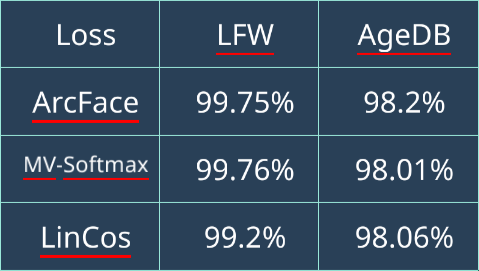
\includegraphics[width={0.25\textwidth}]{results}
    		\caption{Results}
	\end{figure}
\section{Problem formulation}
As we can see that all of the above papers already give a pretty good accuracy, it is pretty impossible to choose the best one. However, due to ease of implementation and familiarity with Pytorch, I chose to proceed with ArcFace. Various experiments can be done with the above methods. One of them is to combine the ideas of LinCos and ArcFace. We can approximate cos($\theta$ + m) (where m = Marginal Penalty) using the method proposed in LinCos paper and reduce the problem of over-fitting. Another possible work-around is to replace cosine with the tangent.
\section{Conclusion}
To conclude, there has been extensive research in the field of face recognition. Due to this, many proposed models have already achieved an accuracy that is possibly less only by the Bayes error. However, there is still room for experimentation, and my focus will remain on trying the above-proposed experiments.
